\documentclass[tikz,border=10pt]{standalone}
\begin{document}
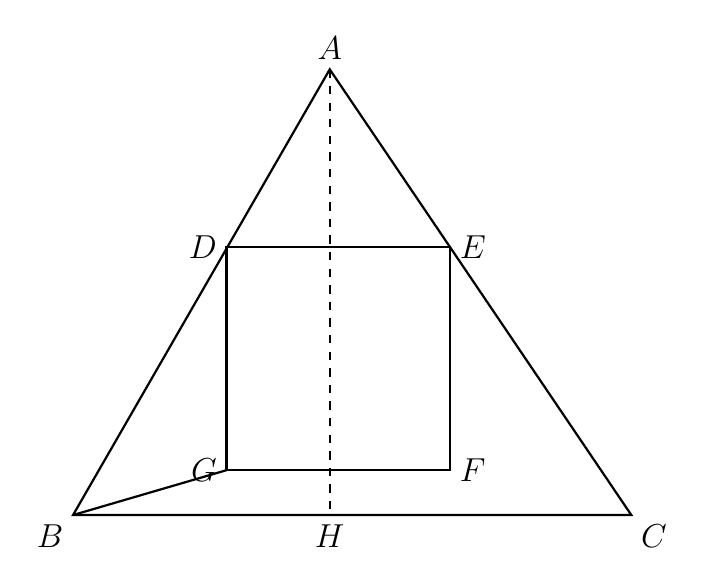
\begin{tikzpicture}[scale=1, every node/.style={font=\large}]
  \coordinate (A) at (4.46,5.66);
  \coordinate (B) at (1.20,0);
  \coordinate (C) at (8.29,0);
  \coordinate (D) at (3.15,3.40);
  \coordinate (E) at (5.99,3.40);
  \coordinate (F) at (5.99,0.57);
  \coordinate (G) at (3.15,0.57);
  \coordinate (H) at (4.46,0);

  \draw[thick] (A) -- (B) -- (C) -- cycle;
  \draw[thick] (D) -- (E) -- (F) -- (G) -- cycle;
  \draw[thick] (B) -- (G);
  \draw[dashed,thick] (A) -- (H);

  \node[above] at (A) {$A$};
  \node[left] at (D) {$D$};
  \node[right] at (E) {$E$};
  \node[right] at (F) {$F$};
  \node[left] at (G) {$G$};
  \node[below left] at (B) {$B$};
  \node[below right] at (C) {$C$};
  \node[below] at (H) {$H$};
\end{tikzpicture}
\end{document}
